%!TEX root = ../thesis.tex
%*******************************************************************************
%****************************** Third Chapter **********************************
%*******************************************************************************

\chapter{Method}
\label{chapter:method}

% **************************** Define Graphics Path **************************
\graphicspath{{../img/thesis/}{../img/plots/vae_latents/}{../img/related_works/}}

\par
In this chapter, we describe the models we use to demonstrate the efficiency of the
general lossy compression framework developed in Section
\ref{sec:compression_without_quantization}. We begin by describing the input
pipeline, followed by our model architectures and their training procedure. We
then present 3 tractable, coded sampling algorithms that can be used within our
framework.

Based on our framework, at a high level our image compression algorithm is as
follows:

\begin{framed}
\begin{enumerate}
\item Pick an appropriate VAE-based architecture (Probabilistic Ladder Networks
  (PLNs) in our case) for image reconstruction. (Section \ref{sec:architectures})

\item Train the model on a reasonably selected dataset for this task. (Sections
  \ref{sec:dataset_preproc} and \ref{sec:architectures})

\item Once the VAE is trained, given a new image
  $\vec{x}$, we can use the latent posterior $q(\vec{z} \mid \vec{x})$ and
  prior $p(\vec{z})$ for our coded sampling algorithm. (Section
  \ref{sec:coded_sampling})

\item We may consider using entropy codes to further increase the efficiency of
  our coding, if appropriate. 

\end{enumerate}
\end{framed}

\par
A rather pleasing aspect of this is the modularity that is allowed by the
removal of quantization from the training pipeline: our method is reusable with
virtually any regular VAE architecture, which opens up the possibility of
creating efficient compression algorithms for any domain where a VAE can be used
to reconstruct the objects of interest. 

\section{Dataset and Preprocessing}
\label{sec:dataset_preproc}
\par
We trained our models on the CLIC 2018 dataset (\cite{clic2018}), as it seemed
sufficiently extensive for our project. It was also curated for an image
compression challenge, and thus ``bad'' images have been
filtered out, which reduced the amount of preprocessing required on our side.
\par
The dataset contains high-resolution PNG encoded photographs, 585 in the
training set and 41 photos in the validation set. The test set is not
publicly available, as it was reserved for the competition. 
To make training tractable, similarly to previous works, we randomly extracted
$256 \times 256$ pixel patches from each image. The number of patches $P$ was
based on their size of the image, according to the formula
\[
  P(W, H) = C \times \left \lfloor \frac{W}{256} \right \rfloor \times
  \left \lfloor \frac{H}{256} \right \rfloor,
\]
where $W, H$ are the width and height of the current image, respectively and $C$
is an integer constant we set. We used $C = 15$, which yielded us a training set
of 93085 patches.
\par
We note that all image data we used for learning was in RGB format. It is
possible to achieve better compression rates using the YCbCr format
(\cite{balle2016end}, \cite{rippel2017real}), however, for simplicity's sake as
well as due to time constraints we leave investigating this for later work.
\section{Architectures}
\label{sec:architectures}
\par
In this section, we describe the various architectures that we experimented with.
The basis of all our architectures was inspired by the ones used in
\cite{balle2016end} and \cite{balle2018variational}. In particular, we use the
General Divisive Normalization (GDN) layer for encoding and its approximate
inverse, the IGDN layer for decoding (\cite{balle2015density}, \cite{balle2016end}).

\subsection{VAEs}
\label{sec:method_vaes}
\par
As a baseline, we started by replicating the exact architecture
presented in \cite{balle2016end} but using a Gaussian prior and posterior
instead. We chose mirror padding with our convolutions, as it is standard
for in this setting (\cite{theis2017lossy}). Luckily, the most
error-prone part, the implementation of the GDN and IGDN layers was already
available in \texttt{Tensorflow}\footnotemark.

\par While VAEs are by now fairly standard and we assume that the reader is at
least somewhat familiar with them, our later models build on them and are
non-standard, hence it is useful to briefly go over them and introduce
notation that we extend in the following sections.

\footnotetext{\url{https://www.tensorflow.org/api_docs/python/tf/contrib/layers/gdn}}

\paragraph{Note:} In the following, we will assume that all multivariate
distributions have diagonal covariance structure, and hence we
parameterize their scales using vectors, to be understood as the diagonal of the
covariance matrix. Furthermore, In the case of Gaussians, in this section only
we parameterize them using their standard deviations instead of their variances.
All arithmetic operations on vectors are also to be understood elementwise.

\begin{figure}
  \centering
  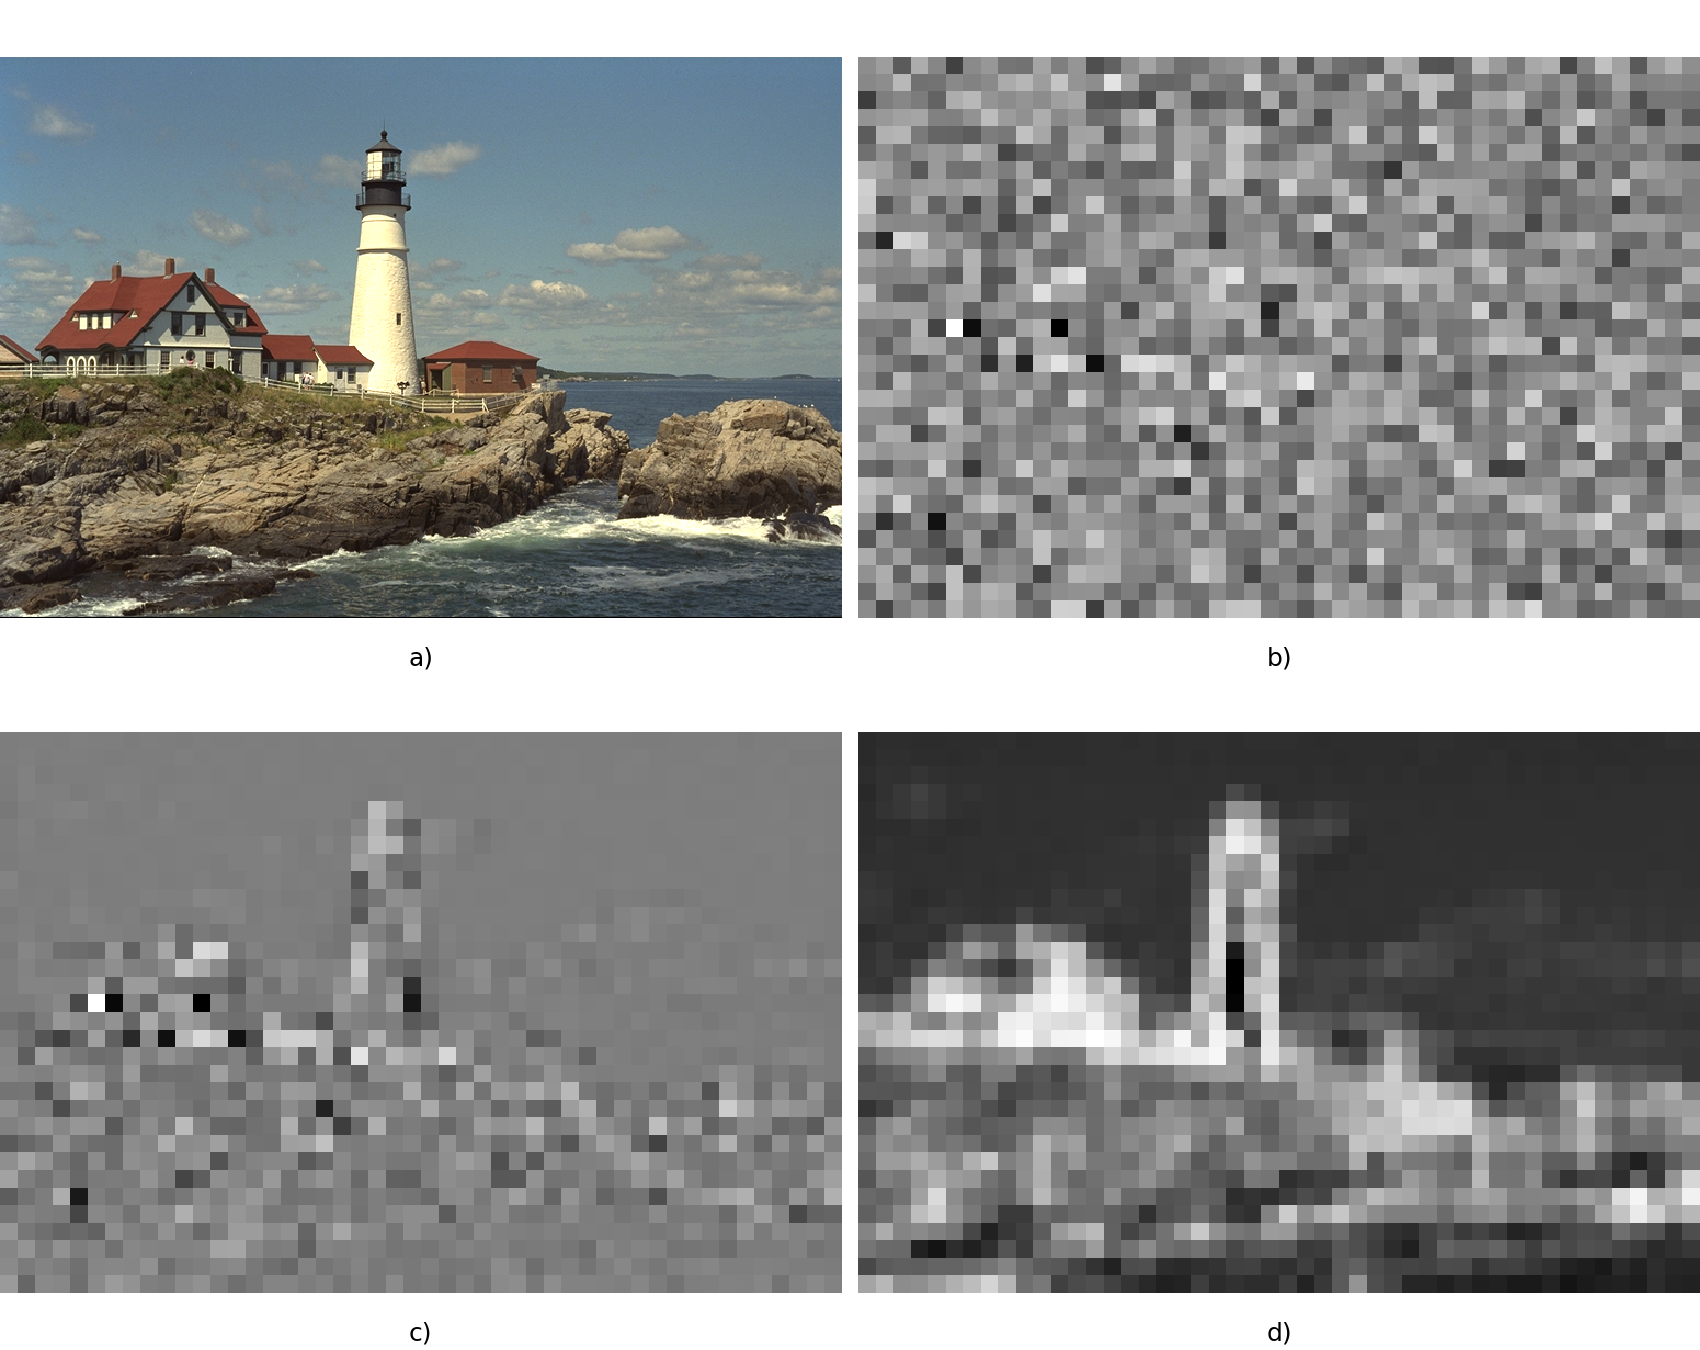
\includegraphics[width=\textwidth]{vae_rand_posterior.png}
  \caption[Latent spaces induced by \texttt{kodim21} in our VAE.]
  {\textbf{a)} \texttt{kodim21.png} from the Kodak Dataset. \textbf{b)}
    A random sample from the VAE posterior. \textbf{c)} Posterior means in a
  randomly selected channel. \textbf{d)} Posterior standard deviations in the same
  randomly selected channel. We can see that there is a lot of structure in the
  latent space, on which the full independence assumption will have a detrimental
  effect. (We have examined several random channels and observed the
  similarly high structure. We present the above cross-section without preference.)}
  \label{fig:vae_rand_posterior}
\end{figure}

\paragraph{}
In a regular VAE, we have a first-level encoder, that given some input
$\vec{x}$ predicts the posterior
\[
  q^{(1)}(\vec{z}^{(1)} \mid \vec{x}) = \Norm{\vec{z}^{(1)} \mid
  \MU^{e, (1)}(\vec{x}), \SIGMA^{e, (1)}(\vec{x})},
\]
where $\MU^{e, (1)}(\vec{x}) = (m \circ f)(\vec{x})$ predicts the mean and
$\SIGMA^{e, (1)}(\vec{x}) = (\exp \circ s \circ f)(\vec{x})$ predicts the
standard deviation of the posterior. Here $f$ is a highly nonlinear mapping of
the input; in reality corresponding to several layers of neural network
layers. Notice that $f$ is shared for the two statistics. Then, $m$ and $s$ are
custom linear transformations, and finally, we take the exponential of $s \circ f
$ to force the standard deviation to be positive. We sample $\tilde{\vec{z}}^{(1)}
\sim q^{(1)}$. We show a typical posterior distribution given an image in Figure
\ref{fig:vae_rand_posterior}.
The first level prior is usually assumed to be a diagonal Gaussian
\[
  p^{(1)}(\vec{z}^{(1)})  = \Norm{\vec{z}^{(1)} \mid \vec{0}, I}.
\]
Finally, the first level decoder predicts the statistics of the data likelihood,
\[
  p(\vec{x} \mid \tilde{\vec{z}}^{(1)}).
\]

\paragraph{A note on the latent distributions} We have chosen to use Gaussian
latent distributions due to their simplicity, as well as their extensibility to
PLNs (see Section \ref{sec:prob_ladder_networks}). On the other hand, we note
that Gaussians are inappropriate, as it has been shown that the filter responses
of natural images usually follow a heavy-tailed distribution, usually assumed to
be a Laplacian (\cite{jain1989fundamentals}), as used directly in
(\cite{clic2018winner}), but can also be approximated reasonably well by Gaussian
Scale Mixtures (\cite{portilla2003image}), as adopted by \cite{theis2017lossy}.
While it would be interesting to investigate incorporating these into our
model, as they do not extend trivially to our more complex model settings (in
particular PLNs, as we formulated them here require the latent posterior
distribution's family to be self-conjugate), we leave this for future work.




\subsection{Data Likelihood and Training Objective}
\begin{figure}
  \centering
  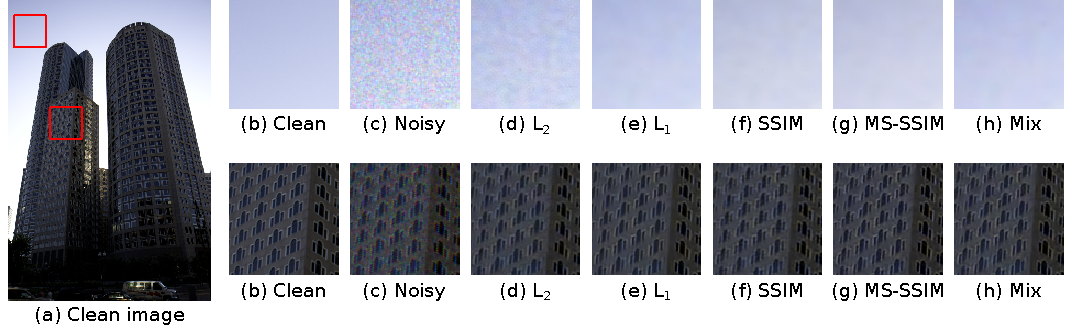
\includegraphics[width=\textwidth]{zhao_loss_comparison.pdf}
  \caption[Loss comparison for neural image reconstruction.]
  {Image reconstruction quality comparison on the task of joint
    image denoising and demosaicing, for the same architecture optimized using
    different distortion metrics. \textbf{a)-b)} Show the original image.
    \textbf{c)} Show the input to the networks. \textbf{d) - h)} Show
    reconstructions using various distortion metrics. Mix is (approximately)
    defined as $(1 - \lambda) L_1 + \lambda \text{MS-SSIM}$ for $\lambda = 0.84$.
    The differences are best
    seen on the electronic version, zoomed in. We can clearly see the patchy
    artefacts introduced by Mean Squared Error (\textbf{d)}), and how much
    better Mean Absolute Error (\textbf{e)}) performs compared to it.
    (Image is taken from \cite{zhao2015loss}. We changed the fonts of their
    captions to a sans-serif font for better readability.)}
  \label{fig:zhao_loss_comparison}
\end{figure}
\par
Based on the framework presented in Section
\ref{sec:compression_without_quantization}, the training objective used to train
the VAE is the (weighted) ELBO:
\begin{equation}
\label{eq:regular_vae_elbo}
\Exp{\log p(\vec{x} \mid \vec{z}^{(1)})}{q^{(1)}(\vec{z}^{(1)})}
- \beta \KL{q^{(1)}(\vec{z}^{(1)} \mid \vec{x})}{p^{(1)}(\vec{z}^{(1)})}.
\end{equation}
As the latent posterior and prior are both Gaussians, the KL can be computed
analytically, and there is no need for a Monte Carlo estimation. A popular and
simple choice for the likelihood to be chosen a Gaussian, in which case the
expectation of the log-likelihood corresponds to the mean squared error
between the original image and its reconstruction. This also corresponds to
optimizing for the PSNR as the perceptual metric. However, PSNR correlates badly
with the Human Visual System (HVS)'s perception of image quality (\cite{girod1993s}
\cite{eskicioglu1994image}). This is mainly because an MSE training objective is
tolerant to small deviations regardless of the structure in the image, and hence
this leads to blurry colour patch artefacts in low-textured regions, which the
HVS quickly picks up as unpleasant. A thorough survey of different
training losses for image reconstruction was performed by
\cite{zhao2015loss}, see Figure \ref{fig:zhao_loss_comparison}. Optimizing the
MS-SSIM distortion for the same architecture, they show that the artefacts are
greatly reduced. They also show that, somewhat surprisingly, Mean Absolute Error
(MAE) also significantly reduces and in some cases completely removes the
unpleasant artefacts introduced by MSE.
This is because MAE no longer underestimates small deviations, at the cost of
somewhat blurrier edges, which MSE penalized more. The MAE corresponds to a
diagonal Laplacian log-likelihood with unit scale, which is what we decided to
use in our experiments. This results in efficient training (an MS-SSIM
training loss, though differentiable, is very expensive to compute) as well as
it will enable us to use a further enhancement, see Section
\ref{sec:learn_gamma}.

Concretely, our likelihood is going to be
\begin{equation}
\label{eq:laplace_likelihood}
  p(\vec{x} \mid \vec{z}^{(1)}) = \Laplace{\hat{\vec{x}} \mid
  \MU^{d, (1)}(\tilde{\vec{z}}^{(1)}), I},
\end{equation}
where $\MU^{d, (1)}$ is the reverse operation of $\MU^{e, (1)}$.


\subsection{Probabilistic Ladder Network}
\label{sec:prob_ladder_networks}

\begin{figure}
  \centering
  \includegraphics[width=\textwidth]{VAE_architecture.png}
  \caption[Our Probabilistic Ladder Network (PLNl) architecture.]
  {PLN network architecture. The blocks signal data transformations, the
    arrows signal the flow of information. \textbf{Block descriptions:}
    \textit{Conv2D:} 2D convolutions along the spatial dimensions, where the
    $W\times H \times C / S$ implies a $W \times H$ convolution kernel, with $C$
  target channels and $S$ gives the downsampling rate (given a preceding letter
  ``d'') or the upsampling rate (given a preceding letter ``u''). If the slash
  is missing, it means that there is no up/downsampling. All convolutions operate
  in \texttt{same} mode with mirror padding. \textit{GDN / IGDN:} these are the
  non-linearities described in \cite{balle2016end}. \textit{Leaky ReLU:}
  elementwise non-linearity defined as $\max\{x, \alpha x\}$, where we set
  $\alpha=0.2$. \textit{Sigmoid:} Elementwise non-linearity defined as
  $\frac{1}{1 + \exp\{-x\}}$. We ran all
  experiments presented here with $N = 196, M = 128, F = 128, G = 24$.}
  \label{fig:pln_architecture}
\end{figure}

\par
We now introduce two extensions of VAEs to accommodate more complex latent
dependency structures: hierarchical VAEs (H-VAEs) and Probabilistic Ladder
Networks (PLNs) (\cite{sonderby2016train}). For simplicity's sake, we only
consider two-level H-VAEs and PLNs, these can be easily extended to more
stochastic levels. In both cases, we essentially stack VAEs on top of each
other and train them together, though the way this is done is crucial for our
use case.

\par
To extend the VAE architecture from Section \ref{sec:method_vaes} to get a
2-level H-VAE, once $\tilde{\vec{z}}^{(1)}$ is sampled, we use it to predict
the statistics of the second level posterior
\[
  q^{(2)}(\vec{z}^{(2)} \mid \tilde{\vec{z}}^{(1)}) = \Norm{\vec{z}^{(2)} \mid 
  \MU^{e, (2)}(\tilde{\vec{z}}^{(1)}), \SIGMA^{e, (2)}(\tilde{\vec{z}}^{(1)})},
\]
where $\MU^{e, (2)}(\tilde{\vec{z}}^{(1)})$ and
$\SIGMA^{e, (2)}(\tilde{\vec{z}}^{(1)})$ are analogous to their first level
counterparts. Next the second level is sampled $\tilde{\vec{z}}^{(2)} \sim
q^{(2)}$. The second level prior $p^{(2)}(\vec{z}^{(2)})$ is now the diagonal
unit-variance Gaussian, and the first level priors' statistics are predicted
using $\tilde{\vec{z}}^{(2)}$:
\[
  p^{(1)}(\vec{z}^{(1)} \mid \tilde{\vec{z}}^{(2)}) =
  \Norm{\vec{z}^{(1)} \mid \MU^{d, (2)}(\tilde{\vec{z}}^{(2)}),
    \SIGMA^{e, (2)}(\tilde{\vec{z}}^{(2)})}.
\] 
The data likelihood's mean is predicted using $\tilde{\vec{z}}^{(1)}$ as before
(\cite{sonderby2016train}).
\par
The issue with H-VAEs is that the flow of information is limited by the
bottleneck of the final stochastic layer. PLNs resolve this issue by allowing
the flow of information between lower levels as well. To arrive at them, we
make the following modification to our H-VAE: first, once $q^{(1)}$ is known,
instead of sampling it immediately, we instead use its mean to predict the
statistics of the second level posterior:
\[
  q^{(2)}(\vec{z}^{(2)} \mid \tilde{\vec{z}}^{(1)}) = \Norm{\vec{z}^{(2)} \mid 
  \MU^{e, (2)}(\MU_{\vec{x}}), \SIGMA^{e, (2)}(\MU_{\vec{x}})},
\]
where $\MU_{\vec{x}} = \MU^{e, (1)}(\vec{x})$. Now, $\tilde{\vec{z}}^{(2)} \sim
q^{(2)}$ is sampled. The first level prior $p^{(1)}$ is calculated as before.
Finally, we allow the flow information on the first level by setting the
posterior $q^{(1)}$ as the combination of the statistics predicted on the first
level from the data and the statistics of $p^{(1)}$, inspired by the
self-conjugacy of the Normal distribution in Bayesian inference\footnotemark:
\[
  q^{(1)}(\tilde{\vec{z}}^{(1)} \mid \tilde{\vec{z}}^{2}, \vec{x}) =
  \Norm{\tilde{\vec{z}}^{(1)} \,\bigg|\,
    \frac{\SIGMA_{\vec{z}^{(1)}}^{-2} \MU_{\vec{x}} + \SIGMA_{\vec{x}}^{-2}
      \MU_{\vec{z}^{(1)}}}{\SIGMA_{\vec{x}}^{-2} + \SIGMA_{\vec{z}^{(1)}}^{-2}
    },
  \frac{1}{\sqrt{\SIGMA_{\vec{x}}^{-2} + \SIGMA_{\vec{z}^{(1)}}^{-2} }}},
\]
where $\MU_{\vec{x}} = \MU^{e, (1)}(\vec{x}), \MU_{\vec{z}^{(1)}} = \MU^{d, (2)}(\tilde{\vec{z}}^{(2)})$
and $\SIGMA_{\vec{x}} = \SIGMA^{e, (1)}(\vec{x}), \SIGMA_{\vec{z}^{(1)}} = \SIGMA^{d, (2)}(\tilde{\vec{z}}^{(2)})$.
We sample $\tilde{\vec{z}}^{(1)} \sim q^{(1)}(\tilde{\vec{z}}^{(1)} \mid
\tilde{\vec{z}}^{(2)}, \vec{x})$, and predict the mean of the likelihood using it.
\par 
The reason why H-VAEs and PLNs are more powerful models than regular VAEs, is
because regular VAEs make an independence assumption between the latents to make
the model tractable to compute, while H-VAEs and PLNs relax this to a
\textit{conditional independence} assumption. In this sense, the architecture of 
\cite{balle2018variational} also defines a PLN. We present the PLN architecture
we used in our experiments in Figure \ref{fig:pln_architecture}. We demonstrate
the power of conditional independence in PLNs compared to the full independence
assumption in Figure \ref{fig:ladder_rand_posterior}.

\footnotetext{We note that the formula we used in our definition is the actual
  combination rule for a Gaussian likelihood and Gaussian prior. The formula given in
  \cite{sonderby2016train} is slightly different. We are not sure if it is a
  typo or it is what they actually used. We found our combination rule worked
  quite well in practice.}

\begin{figure}
  \centering
  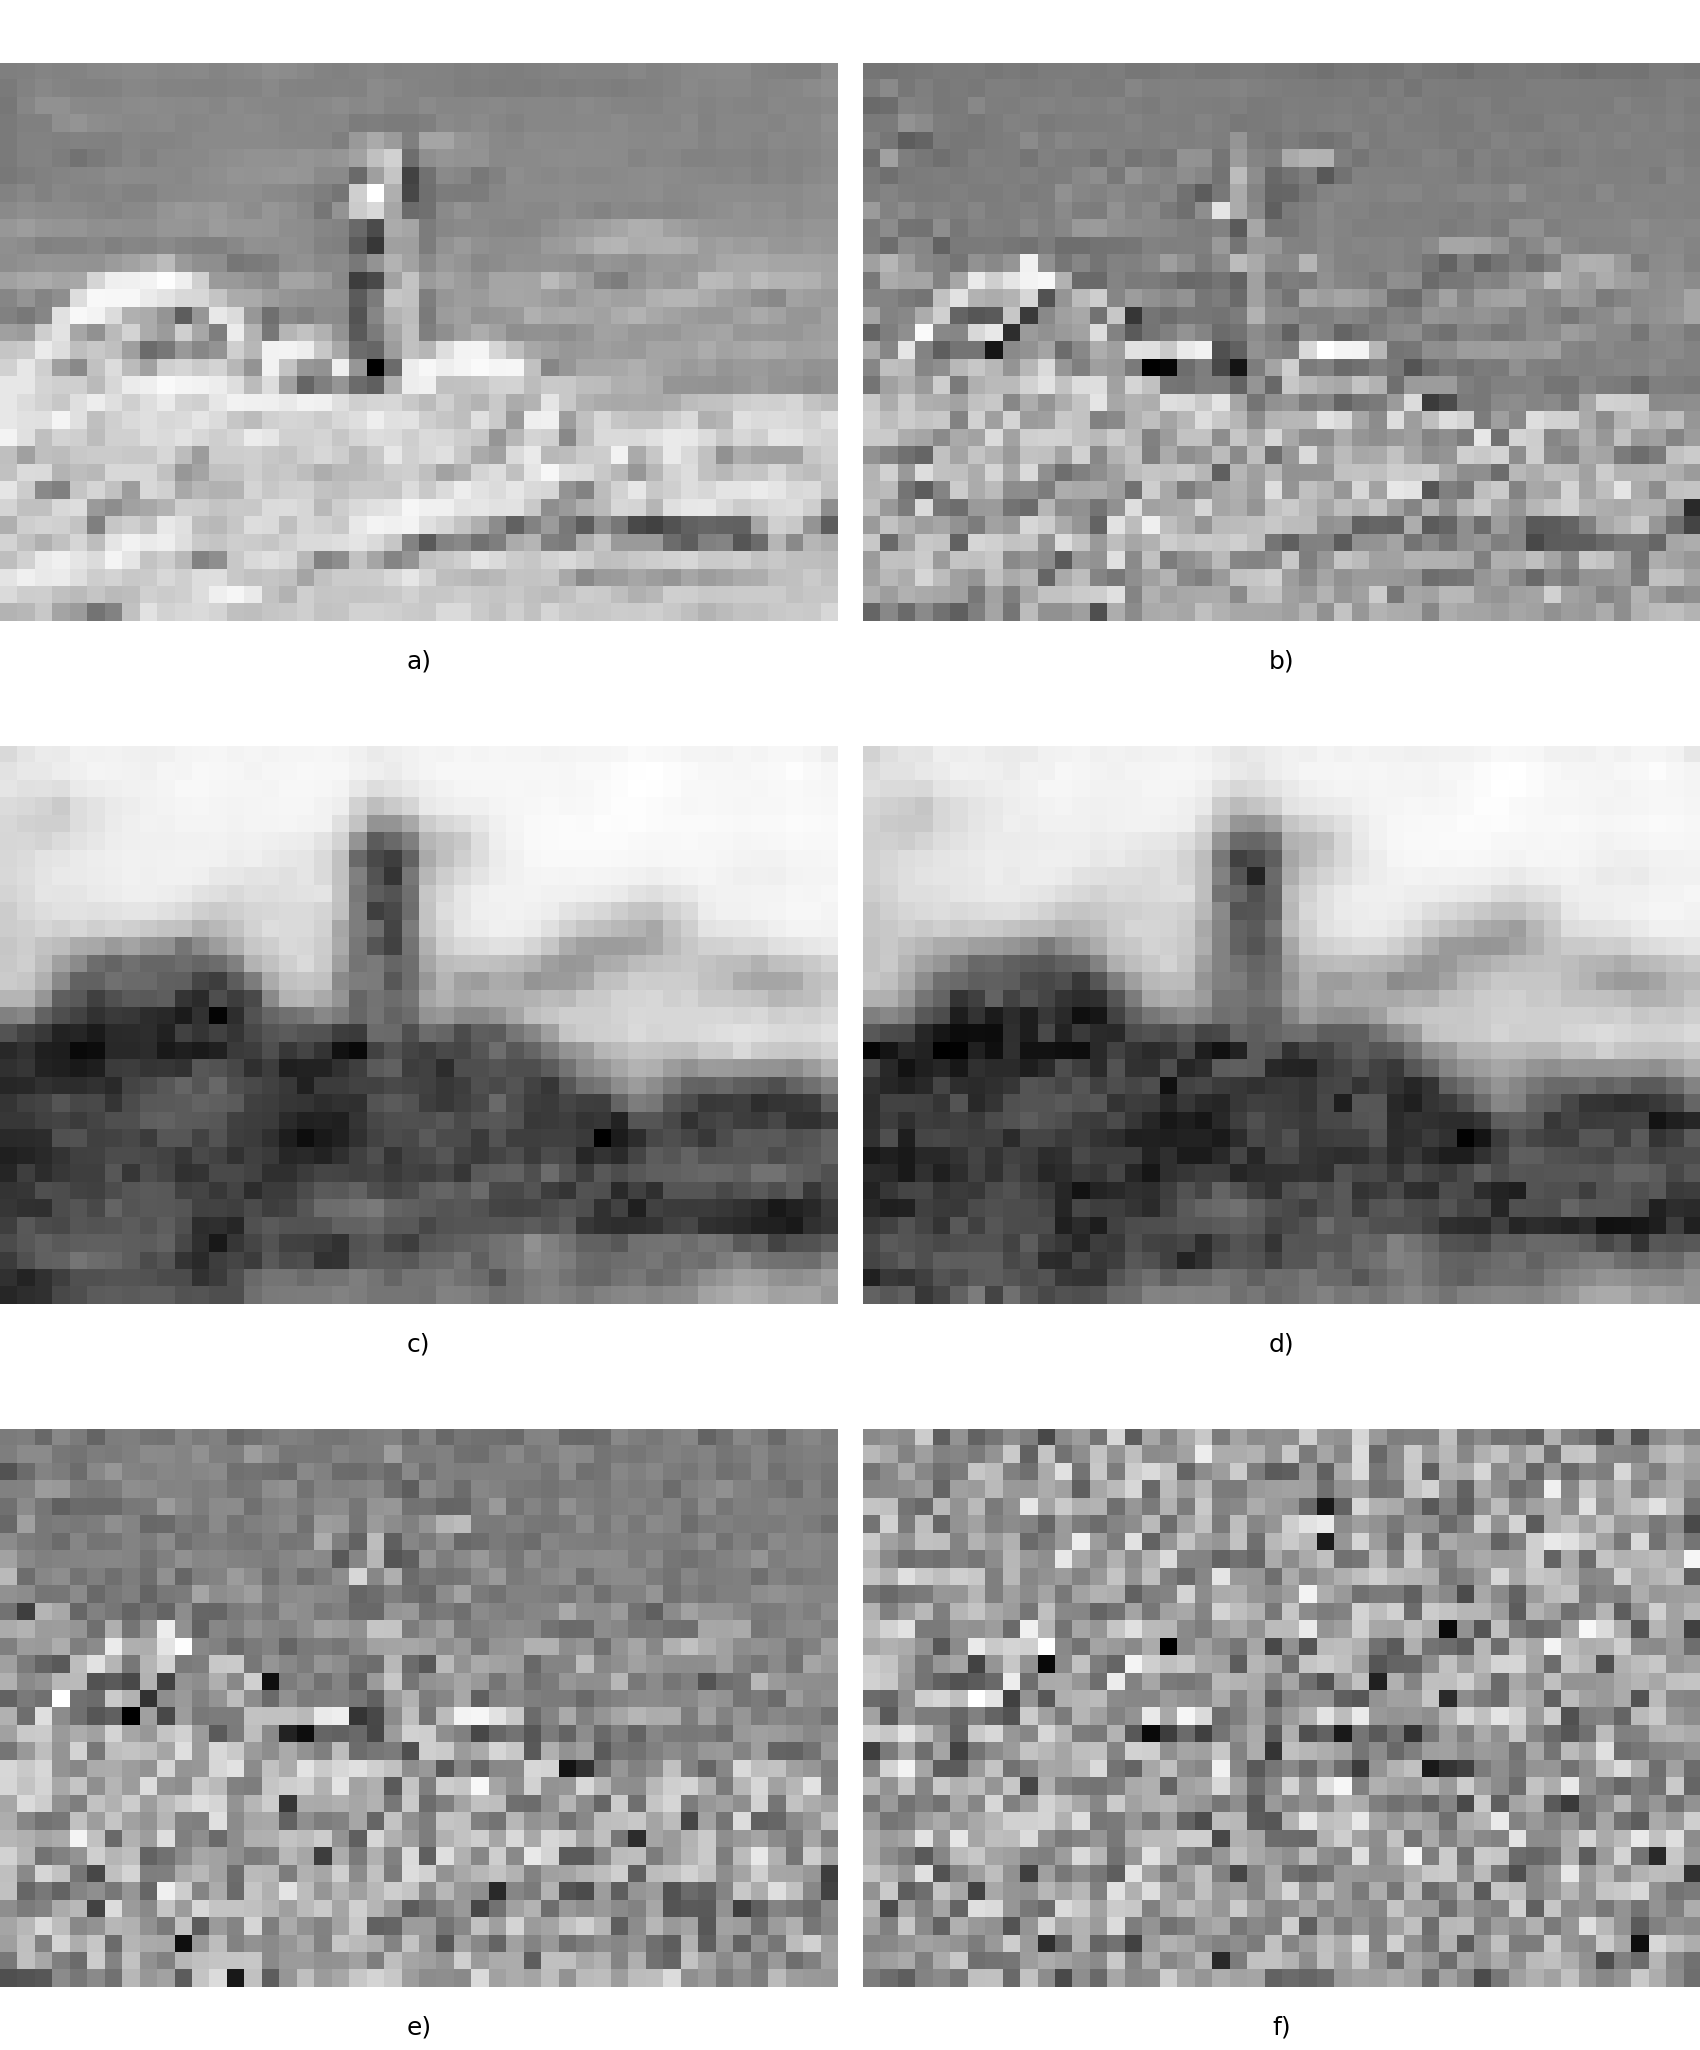
\includegraphics[width=\textwidth]{ladder_rand_posterior.png}
  \caption[Latent spaces induced by \texttt{kodim21} in our PLN]
  {We continue the analysis of the latent spaces induced by
    \texttt{kodim21} from the Kodak Dataset. Akin to Figure
    \ref{fig:vae_rand_posterior}, we have selected a random channel for both the
    first and second levels each and present the spatial cross-sections along these
    channels. \textbf{a)} Level 1 prior means. \textbf{b)} Level 1 posterior means.
    \textbf{c)} Level 1 prior standard deviations. \textbf{d)} Level 1 posterior
    standard deviations. \textbf{e)} Random sample from the Level 1 posterior.
    \textbf{f)} The sample from \textbf{e)} standardized according to the level
    1 prior. Most structure from the sample is removed, hence we see that the
    second level has successfully learned a lot of the dependencies between the
    latents. We have checked cross-sections along several randomly selected
    channels and observed the same phenomenon. We present the above with no preference.}
  \label{fig:ladder_rand_posterior}
\end{figure}

\paragraph{}
Finally, we need to update the regularizing term of the ELBO to incorporate the
joint posterior and priors over the latents. This works out to be
\begin{align*}
  \KL{q(\vec{z}^{(1)}, \vec{z}^{(2)} \mid \vec{x})}{p(\vec{z}^{(1)}, \vec{z}^{(2)})} =\,\,& 
  \KL{q(\vec{z}^{(2)} \mid \vec{x})}{p(\vec{z}^{(2)})} + \\
  &\KL{q(\vec{z}^{(1)} \mid \vec{z}^{(2)} , \vec{x})}{p(\vec{z}^{(1)} \mid \vec{z}^{(2)})},
\end{align*}
which we can also compute analytically.

\section{Training}
\par \cite{sonderby2016train} give two key pieces of advice to train PLNs:
\begin{itemize}
\item Use batch normalization (BN) (\cite{ioffe2015batch}).
\item Use a warmup on the coefficient of the KL term in the loss.
  Concretely, given a target coefficient $\beta_0$, the actual coefficient they
  recommend should be
  \[
    \beta(t) = \min\left\{ \frac{t}{W}, 1 \right\} \times \beta_0,
  \]
  where $t$ is the current iteration and $W$ is the \textit{warmup period}.
\end{itemize} 
We ended up not utilizing point 1, due to an argument of
\cite{balle2018variational}, namely that GDN already performs a similar kind of
normalization as BN, and it did not improve their results. 

\subsection{Learning the Variance of the Likelihood}
\label{sec:learn_gamma}
\par
As we have noted, the reconstructions are blurry.
A solution offered by \cite{dai2019diagnosing} is to introduce a new parameter
$\gamma$ to the model, that will be the scale of the data likelihood. In our
case, since we are using a Laplace likelihood, we will have
\[
  p(\hat{\vec{x}} \mid \vec{z}^{(1)}) = \Laplace{\hat{\vec{x}} \mid \MU^{d,
      (1)}(\tilde{\vec{z}}^{(1)}), \gamma}.
\]
In the case of a Gaussian, $\gamma$ would be the variance of the distribution.
Then, it is suggested that instead of predicting gamma (i.e. using a
heteroscedastic model), or setting it as a hyperparameter, \textit{we learn it}.
In \cite{dai2019diagnosing} this is used in conjunction with another novel
technique to achieve generative results with VAEs that are competitive with
state-of-the-art GANs (\cite{goodfellow2014generative}). In this work, however,
as the second technique is irrelevant to us, we focus on learning $\gamma$ only.
\par
Let us examine this concept a bit more: let $D$ be the (original) log-likelihood
term with unit scale, and $R$ the (original) regularizing term, already
multiplied by our target coefficient $\beta$. Then, our new loss is going to be
\[
  L = \frac{1}{\gamma}D + R.
\]
Multiplying this through by $\gamma$ does not change the minimizer\footnotemark of the
expression, but we get the new loss
\[
  L' = D + \gamma R.
\]
\cite{dai2019diagnosing} show that if $\gamma$ is learned, then under some mild
assumptions $\gamma \rightarrow 0$ as $t \rightarrow \infty$ (where $t$ is the
number of iterations in the training procedure). This means that if we set some
target $\gamma_\infty$, and use
\[
  \gamma' = \max\{ \gamma, \gamma_\infty \},
\]
as the scale of the data likelihood, we get a dual effect to the warmup
recommended by \cite{sonderby2016train}, but with automatic scaling.
\footnotetext{\url{https://openreview.net/forum?id=B1e0X3C9tQ&noteId=ByeNgv9KTQ}}
\par
In practice, $\gamma$ does not converge to 0, but to a number very close to
zero, which in experiments was around $\approx 0.02$, and hence instead of using
$\gamma'$, we set different $\beta$s to achieve different rate-distortion
results. From now on, we will refer to PLNs where we also learned $\gamma$ as
$\gamma$-PLNs. In Figure \ref{fig:gamma_rand_posterior} we show the posterior of 
one of our $\gamma$-PLNs.
\begin{figure}
  \centering
  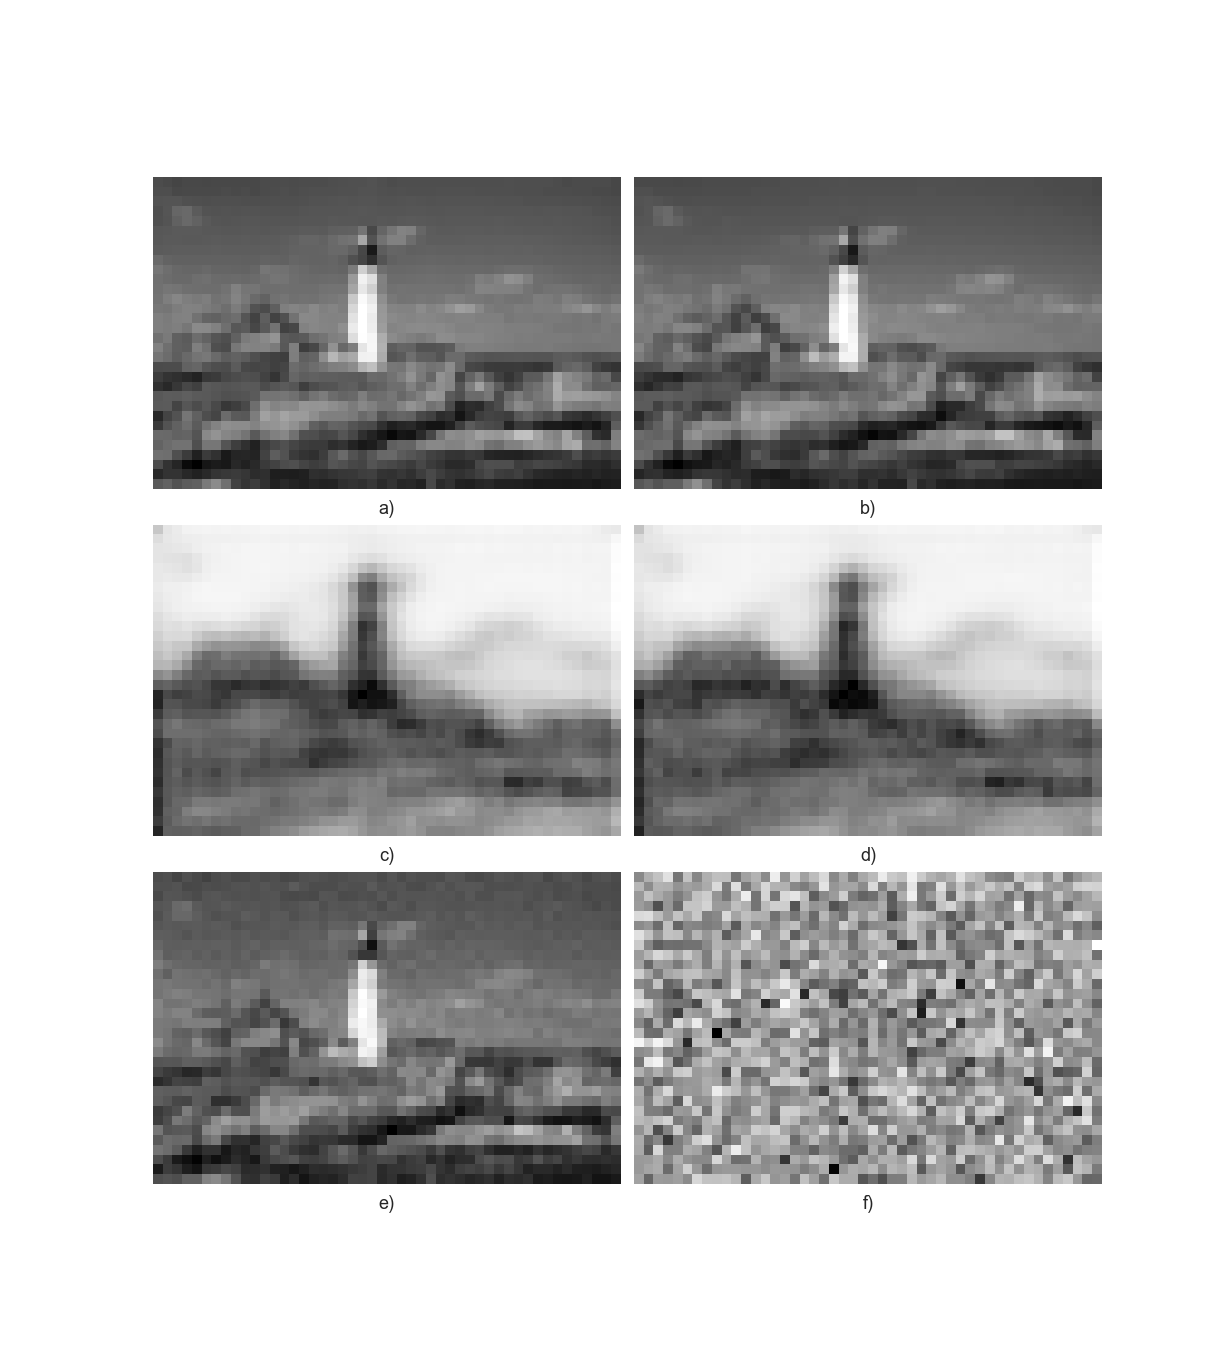
\includegraphics[width=\textwidth]{gamma_rand_posterior.png}
  \caption[Latent spaces induced by \texttt{kodim21} in our $\gamma$-PLN.]
  {We continue the analysis of the latent spaces induced by
    \texttt{kodim21} from the Kodak Dataset. Akin to Figures
    \ref{fig:vae_rand_posterior} and \ref{fig:ladder_rand_posterior},
    we have selected a random channel for both the
    first and second levels each and present the spatial cross-sections along these
    channels. \textbf{a)} Level 1 prior means. \textbf{b)} Level 1 posterior means.
    \textbf{c)} Level 1 prior standard deviations. \textbf{d)} Level 1 posterior
    standard deviations. \textbf{e)} Random sample from the Level 1 posterior.
    \textbf{f)} The sample from \textbf{e)} standardized according to the level
    1 prior. We observe the same phenomenon, with no significant difference, as
    in Figure \ref{fig:ladder_rand_posterior}. We note that while the posterior
    sample may seem like it has more significant structure than the one in the
    previous Figure. This is only coincidence; some of the regular PLN's
    channels contain similar structure, and some of the $\gamma$-PLN's channels
    contain more noisy elements.
  }
  \label{fig:gamma_rand_posterior}
\end{figure}

\section{Sampling and Coding}
\label{sec:coded_sampling}
\par
Once the appropriate network has been trained, this means that for any image $\vec{x}$
we are able to produce a latent posterior $q(\vec{z} \mid \vec{x})$ and prior
$p(\vec{z})$. The next step in our framework is to use a bits-back efficient coded sampling
algorithm to code a sample from the posterior. The first practical coded
sampling algorithm to was described in \cite{havasi2018minimal}, but there
are several key differences between our setting and theirs:

\begin{itemize}
\item \textbf{Variable sized latent space:} The original method was
  developed for compressing the weight distribution of a BNN, whose dimension is
  fixed. In our case, due to our fully convolutional architecture, our rendition
  of the algorithm must be able to adapt gracefully to a range of latent space
  dimensions. 

\item \textbf{Different posterior effects:} As our latent spaces will carry much
  more information about the topological nature of the coded image, the
  distribution of informative versus non-informative posteriors and their
  properties will be different from the original setting, and we will need to
  adapt to these effects. These effects can be seen in Figures
  \ref{fig:vae_rand_posterior}, \ref{fig:ladder_rand_posterior} and
  \ref{fig:gamma_rand_posterior}.

\item \textbf{Practicality / Resource efficiency:} Since the original method has
  been proposed to compress neural networks after they have been trained, the
  algorithm was proposed with people who have sufficient resources to train them
  in mind. In particular, the original method incorporates several rounds of
  incremental retraining during the compression process to maintain low distortion, which
  might require several GPU hours to complete. As our aim in this work to
  present a practical, universal compression algorithm, we must also design our
  method with a much broader audience in mind. Though we still assume the
  presence of a GPU, our requirements and coding times are much lighter than
  that of the original work.
\end{itemize}

In the rest of this section, we present the ways we addressed the above points.

\subsection{Parallelized Rejection Sampling and Arithmetic Coding}

\paragraph{Sampling}
As a baseline, we designed a parallelized version of Algorithm
\ref{alg:harsha_rej_sampling}, the original bits-back efficient sampling
algorithm presented by \cite{harsha2007communication}. As pointed out by
\cite{havasi2018minimal}, this algorithm quickly becomes intractable once
we leave the univariate setting. Fortunately, as we are working with
(conditional) independence assumptions between the latents, 
sampling each dimension individually and then concatenating them will also
give an exact multivariate sample.

\begin{algorithm}
  \caption{Parallelized, bit-budgeted rejection sampling based on Algorithm
    \ref{alg:harsha_rej_sampling}.}
  \label{alg:multivariate_rej_samp}
  \begin{algorithmic}
    \State \textbf{Inputs:}
    \State $B$ - Bit budget for coding the rejection sample indices
    \State $P$ - Prior probability mass function
    \State $Q$ - Posterior probability mass function
    \State $\langle x_i \sim Q \mid i \in \Nats \rangle$ - Sequence of random draws
    from $Q$
    \Statex
    \Procedure{Rej-Sampler}{$B, P, Q, \langle x_i \sim Q \mid i \in \Nats \rangle$}
    \State $D \gets \text{dim}(P)$
    \State $p_{d, 0}(x) \gets 0 \quad \forall x \in \X, \forall d = 1,\hdots D$.
    \State $p_{d, 0}^* \gets 0, \forall d = 1,\hdots D$.
    \State $A = \vec{0} \in \{0, 1\}^D$
    \Comment Keeps track of whether a dimension has been accepted or not

    \State $S = \vec{0} \in \Reals^D$
    \Comment Sample we are ``building''

    \State $I = -\vec{1} \in \Nats^D$
    \Comment Index vector for each dimension

    \For{$i \gets 1, \hdots 2^B$}

    \For{$d \gets 1, \hdots D$}

    \If{$A_d = 1$}

    \State Skip

    \EndIf


    \State
    $\alpha_{d, i}(x) \gets \min{P_d(x) - p_{d, i - 1}(x), (1 - p_{d, i - 1}^*)Q_d(x)}\quad
    \forall x \in \X$

    \State $p_{d, i}(x) \gets p_{d, i - 1}(x) + \alpha_{d, i}(x)$
    
    \State $p_{d, i}^* \gets \sum_{x \in \X}p_{d, i}(x)$

    \State $\beta_{d, i}(x_i) \gets \frac{\alpha_{d, i}(x)}{(1 - p_{d, i}^*)Q_d(x)}$

    \State Draw $u \sim \Unif{0, 1}$

    \If{$u < \beta_{d, i}(x_i)$}

    \State $A_d \gets 1$
    \Comment Indicate we accepted the sample

    \State $S_d \gets x_i$
    \State $I_d \gets i$

    \EndIf
    
    \EndFor
    \EndFor

    \State Draw $S' \sim Q_{\text{where } I = -1}$
    \Comment Sample dimensions where we have not accepted.

    \State $S_{\text{where } I = -1} \gets S'$
    \Comment Set the ``built'' sample's missing dimensions to $S'$.

    \State $I_{\text{where } I = -1} \gets $ \Call{Quantize}{$S', 16$}
    \Statex
    \Comment Set the missing dims. of $I$ to $S'$ quantized to 16 bits. 

    \State\Return $I, S$
    \EndProcedure
  \end{algorithmic}
\end{algorithm}

\par
We modify Algorithm \ref{alg:harsha_rej_sampling} in two ways to make it more
efficient. While their algorithm is Las Vegas, i.e. it always gives the right
answer, but in random time, this can get very inefficient if we have a few
dimensions with very high KL divergence. We circumvent this issue and fix the
runtime of the algorithm by allocating a bit budget $B$ to each dimension, and
only allowing $2^B$ samples to be examined. If the sample is accepted within
these draws, then we have a code for them. The dimensions where all $2^B$ samples were
rejected, we sample from the target $q$, and quantize the samples to 16 bits.
This gave about a 1\% increase in size at a much-improved runtime. In
particular, for dimensions with KL larger than 16 bits, this is more
efficient than coding them with Algorithm \ref{alg:harsha_rej_sampling}.
We then use the quantized samples as code. The concrete details can be seen in Algorithm
\ref{alg:multivariate_rej_samp}. Instead of using the density of the posterior
and the prior to sample, we finely quantized them and used the probability
masses in the algorithm.

% why doesnt rejection sampling work exactly?
% - the cost is not arising from bad independence assumptions, because we have
%   indepenedence
% - so does it come from a bad match of the actual image posteriors?

\paragraph{Coding}
Simply writing the codes of the individual dimensions given by the rejection
sampler would be very inefficient, because without additional assumptions the
way to uniquely decode them would be to block code them (i.e. code all indices
in 8 bits, say). This would, however, add an $\Oh(1)$ cost per dimension on
the coding length, which is very undesirable. Hence, we implemented a simple
non-adaptive arithmetic coder (\cite{rissanen1981universal}) to mitigate this issue.
Probabilities for the symbol table have been estimated by encoding the entire
CLIC training set and using the empirical probability distribution on the
indices. We used Laplace/additive smoothing for unseen indices (\cite{chen1999empirical}).
In particular, given the empirical distribution of the sample indices $P$,
the probability distribution used is
\[
  \tilde{P}(i) = \begin{cases}
    (1 - \alpha)P(i) & \text{if } i \in I \\
    \frac{\alpha}{N} & \text{otherwise}
    \end{cases}
\]
where $I = \{i \in \Nats \mid P(i) > 0\}$.
In our case we allocated $B = 8$ bits for each individual dimension,
$I = \{0, \hdots 255\}$ as all codable indices appeared. Since we quantized the
outliers to 16 bits, $N = 2^{16} - 2^{8}$. We found that choosing $\alpha
\approx 0.01$ gave the best results.

\paragraph{A note on the Arithmetic Coder}
\par
While for small alphabets the naive implementation of the arithmetic coder is
very fast, the decoding time grows as $\Oh(|\A|)$ in the size of the
alphabet. In particular, decoding the arithmetic code of a reasonably large
image would take up to 30 minutes using the naive implementation on a CPU. The
inefficiency is due to a bottleneck where we need to find in a partition of $[0,
1]$ into which the currently coded interval fits. The naive
uses a linear search over the partitions. This can be made more efficient by
using height-balanced binary search trees (BSTs). In particular, we need to find
the least upper bounding item in the BST for the given point, which can be done
in $\Oh(\log_2|\A|)$ time.
Using this additional trick, we can decode large images' code in a few seconds.
In particular, we implemented an AVL-tree to serve as the BST, which is always
guaranteed to be height-balanced (\cite{adel1962algorithm}).

\paragraph{Issues} Theorem \ref{thm:bits-back_efficiency} guarantees that the
MDL of a realization of a random variable $Y$ given $X$ by using Algorithm
\ref{alg:harsha_rej_sampling} is
\[
  L(X) \leq \KL{q(Y \mid X)}{p(Y)} + 2\log\left( \KL{q(Y \mid X)}{p(Y)} + 1
  \right) + c,
\]
for some small constant $c$.
However, to achieve this for the joint latents $\vec{z}$, we would need to
sample them jointly, which is intractable. Instead, we sample the
dimensions individually, which by the same theorem introduces a $D\cdot c$ nat
extra length to the code, where we assumed $\vec{z} \in \Reals^D$. This is
because the constant cost $c$ is now incurred in every dimension. Since in our
case $D$ is usually on the magnitudes of $10^5 - 10^6$ even for small $c$ this
cost becomes non-negligible. In our experiments (not shown here) this lead to coding
efficiencies $2.5 - 3.5$ times worse than the optimal efficiency predicted by Theorem
\ref{thm:bits-back_efficiency} for the whole multivariate sample. This lead us
to abandon rejection sampling early on in the project for more efficient approximate methods,
which we describe below.

\subsection{Greedy Coded Sampling}
\begin{algorithm}
  \caption{Greedy Coded Sampler}
  \label{alg:greedy_sampler}
  \begin{algorithmic}
    \State \textbf{Inputs:}
    \State $K$ - Number of proposal shards
    \State $B$ - Bit budget for coding the seed of individual shards. 
    \State Will result in $2^B$ samples to be examined per shard.
    \State $\MU_p$ - Mean of proposal distribution
    \State $\SIGMA_p^2$ - Variance of proposal distribution
    \State $q$ - Posterior distribution
    \Statex
    \Procedure{Greedy-Sampler}{$K, B, \MU_p, \SIGMA_p^2, q$}

    \State $\tilde{\vec{z}}_0 \gets \vec{0}$
    \Comment Initialize the sample

    \State $I = ()$
    \Comment Initialize the index set to an empty list
    \For{$k = 1, \hdots, K$}

    \State Set random seed of generator to $k$.
    
    \State Draw $\vec{s}_{k, b} \sim \Norm{\frac{\MU_p}{K}, \frac{\SIGMA_p}{K}}
    \quad$ for $b = 1,\hdots,B$
    
    \State $\vec{c}_{k, b} = \tilde{\vec{z}}_{k - 1} + \vec{s}_{k, b}$

    \State $\tilde{\vec{z}}_k \gets \argmax_{\vec{c}_{k, b}} \left\{ \log q(\vec{c}_{k, b}) \right\}$
    \Comment Create new sample

    \State $i_k \gets \argmax_{b} \left\{ \log q(\vec{c}_{k, b}) \right\}$
    \Comment Store the index of the shard sample that we used

    \State Append $i_k$ to $I$.
    
    \EndFor

    \State \Return $\tilde{\vec{z}}_K, I$
    
    \EndProcedure
  \end{algorithmic}
\end{algorithm}
\par
To solve the issue of dimensionality, we need a way to code a sample
drawn from the multivariate distribution. The strategy of the greedy sampler is
to progressively ``build'' a reasonable sample from the posterior. A well-known
fact about Gaussian distributed random variables is that they are
closed under addition. Concretely,
if $X \sim \Norm{\mu_X, \sigma^2_X}, Y \sim \Norm{\mu_Y, \sigma^2_Y}$, then
\[
  X + Y \sim \Norm{\mu_X + \mu_Y, \sigma_X^2 + \sigma_Y^2}.
\]
In the multivariate case assuming they are diagonal, the extension of
the above is straight forward.
Using this, we may now do the following: pick an integer $K$, that
we will call the \textit{number of shards}. Then, given the prior
$p(\vec{z} \mid \MU, \SIGMA^2)$, we can break it up into $K$ equal
shards $p_k\left(\vec{z} \mid \frac{\MU}{K}, \frac{\SIGMA^2}{K}\right)$.
Note, if we assign a different, but pre-agreed sequence of random seeds to each
shard, then each shard sample can be coded in $B$ bits that we can set. Start
with an initial sample $\tilde{\vec{z}}_0 = \vec{0}$ and draw $2^B$
samples $\vec{s}_{1, b}$ from the first shard $p_1$ and create
``candidate samples'' $\vec{c}_{1, b} =
\tilde{\vec{z}}_0 + \vec{s}_{1, b}$ and calculate their log-likelihoods under the
target. Finally, set $\tilde{\vec{z}}_1 = \argmax_{\vec{c}_{1, b}}\log
q(\vec{c}_{1, b})$, and repeat until we reach $\tilde{\vec{z}}_K$, at which
point we return it. Then the returned vector will be approximately from the
target. More precisely, this is a ``guided'' random walk, where we bias the
trajectory towards the median of the distribution. The code of the distribution
is then the codes of the selected shard samples, concatenated. The algorithm is described in
more detail in Algorithm \ref{alg:greedy_sampler}. 

\paragraph{A note on implementation}
We note that empirically the greedy sampler underperforms when the variances of
some priors are small. To ameliorate this, we standardize the prior and scale the
posterior according to the standardization, i.e. we set 
\[
  q'(\vec{z} \mid \vec{x}) = \Norm{\vec{z} \bigg| \frac{\mu_q -
      \mu_p}{\sigma_p}, \frac{\sigma^2_{q}}{\sigma^2_{p}}},
\]
where $\mu_p, \sigma^2_p$ are the statistics of the original prior and $\mu_q,
\sigma^2_q$ are the statistics of the original posterior. We communicate the
approximate sample $\vec{z}'$ from $q'$ instead of $q$. This is not problematic, as
Gaussian distributed random variables are closed under linear transformations,
i.e. given $X \sim \Norm{m, s^2}$, we have
\[
  \alpha X + \beta = Y \sim \Norm{\alpha m + \beta, \alpha^2 s^2}.
\]
Hence, the decoder may recover an approximate sample from $q$, by calculating
$\vec{z} = \sigma_{p} \vec{z}' + \mu_{p}$.
\paragraph{Issues}
While the greedy sampler makes sampling efficient and tractable from the
posterior, it comes at the cost of reduced sample quality. In particular, it
gives blurrier images. This also means that if we use a PLN to compress an
image and we use the greedy technique to code the latents on the second level,
the first level priors' statistics derived from the biased sample will be off,
and $\KL{q(\vec{z}^{(1)} \mid \tilde{\vec{z}}^{(2)}, \vec{x})}{p(\vec{z}^{(1)} \mid
  \tilde{\vec{z}}^{(2)})}$ will be higher. We have verified empirically, that while
using a biased sample on the second level does not degrade image quality
(possibly due to the noise tolerance of PLNs), it does significantly increase
the compression size (by a factor of $1.2 - 1.5$) of the first level, which is
very significant. This motivated the final sampling algorithm presented here,
only used on the second level of our PLNs.

\subsection{Adaptive Importance Sampling}
\begin{algorithm}
  \caption{Adaptive Importance Sampler based on Algorithm
    \ref{alg:miracle_imp_samp}, introduced by \cite{havasi2018minimal}}
  \label{alg:adaptive_importance_sampler}
  \begin{algorithmic}
    \State \textbf{Inputs:}
    \State $K$ - Maximum individual KL allowed
    \State $G$ - Maximum group size
    \State $B$ - Bit budget per group
    \State $P$ - Proposal distribution
    \State $Q$ - Target Distribution
    \State $\langle x_i \sim Q \mid i \in \Nats \rangle$ - Shared sequence of
    random draws from $Q$
    \Statex
    \Procedure{Adaptive-Importance-Sampler}{$K, G, B, P, Q, \langle x_i \sim Q \mid i \in \Nats \rangle$}
    \State $\Gamma \gets ()$
    \Comment Group sizes
    \State $kl_i \gets \KL{Q_i}{P_i} \forall i = 1, \hdots N$
    \Comment Get KLs for each dimension
    \State $OI \gets $ \Call{Where}{$kl_i > K$}
    \Comment Outlier indices in the vector
    \State Sample $O \sim Q_{OI}$
    \State $\hat{O} \gets $ \Call{Quantize}{O}
    \State $Q' \gets Q_{\setminus OI}$
    \Comment Target distribution restricted to the dimensions defined by $OI$.
    \State $P' \gets P_{\setminus OI}$
    \Comment Remove outlier dimensions
    \State $\gamma \gets 0$
    \Comment Current group size
    \State $k \gets 0$
    \Comment Current group KL

    \For{$i \gets 1, \hdots \text{dim}(Q')$}

    \If{$k + kl_i > B$ or $\gamma + 1> G$}

    \State Append $\gamma$ to $\Gamma$
    \State $k \gets kl_i$
    \State $\gamma \gets 1$

    \Else

    \State $k \gets k + kl_i$
    \State $\gamma \gets \gamma + 1$

    \EndIf

    \EndFor

    \State Append $\gamma$ to $\Gamma$
    \Comment Append the last group size

    \State $S = ()$
    \Comment Importance samples for the groups
    \State $I = ()$
    \Comment MIRACLE sample indices
    \State $g \gets 0$
    \Comment Current group index

    \For{$\gamma$ in $\Gamma$}
    \Comment Now importance sample each group

    \State $idx, s \gets$ \Call{Importance-Sample}{$P_{g:g + \gamma}, Q_{g: g +
        \gamma}, \langle x_i \sim Q \mid i \in \Nats \rangle$}
    \State Append $idx$ to $I$
    \State Append $s$ to $S$

    \EndFor

    \State \Return I, S

    \EndProcedure
  \end{algorithmic}
\end{algorithm}
The adaptive importance sampler uses the importance sampler described in
Algorithm \ref{alg:miracle_imp_samp}, introduced by \cite{havasi2018minimal}.
The idea is to use similar block-based importance sampling as proposed in
\cite{havasi2018minimal}. However, unlike them, we allocate the block sizes
dynamically. In particular, we set a bit budget $B$ per group, a maximum group
size $G$ and an individual limit $K$.
We begin by discarding individual dimensions where the KL is larger
than $K$. Then, we flatten the remaining dimensions in raster-scan order and 
iteratively add dimensions into the current group so long as the total KL of the
group reaches either the bit budget $B$ or the number of dimensions added to the
group reaches $G$. At this point, we start with a new group. Once the whole
vector has been partitioned, we importance sample each group using Algorithm 
\ref{alg:miracle_imp_samp}. The removed dimensions are sampled directly from
the posterior and then the samples are quantized to 16 bits. The complete
algorithm can be seen in Algorithm \ref{alg:adaptive_importance_sampler}.
\par
For ease of referral, since we would perform Adaptive Importance Sampling on the
second level, followed by the Greedy Sampling on the first, We will refer to
this way of sample coding as IS-GS.

\paragraph{}
For the importance sampler, the $\Oh(1)$ sampling cost impeding the rejection
sampler is negligible, as it will be now shared across approximately $G$
dimensions. We can also forgo the arithmetic coder, as the indices output by the
sampler are already going to be quite efficient. On the other hand, we also
have to communicate the groups as well. Instead of communicating
group indices, we can instead order the latents and communicate consecutive
group sizes, from which the indices can be easily reconstructed. Each
group's size takes up at most $\lceil \log_2G \rceil$ bits. In total, we usually
get slightly more than $\left\lceil \frac{N_2}{G} \right\rceil$ groups,
(where $N_2$ is the dimensionality of the second level). This is still
very inefficient, but so long as $N_2$ is sufficiently small compared to the
code length for the indices, it will be manageable. We also note that the group
size is likely to be biassed towards higher values, and hence building an
empyrical distribution them and arithmetic coding the sequence could lead to a
big reduction in the inefficiency, however, we found this not to be too
important to focus on. 

\paragraph{Greedy Sampler} It is easy to see that the greedy sampler is already
as efficient as it could be. The sample indices for each shard are as compactly
represented as possible, as we expect the maximum of the samples to be uniformly
distributed. Hence, the only other items that need to be coded is the number
of shards and the number of samples for each shard for the cumulative sample to
be decodable. Hence, for the greedy sampler, we just wrote the indices straight
to the binary file.
